\chapter{ANTECEDENTES Y ESTADO DEL ARTE}
\label{ch:2}
% ==============================================================================================================
\section{Introducción}
\label{ch:2:section:introduction}

El proyecto que desarrollamos se encuentra en una frontera muy difusa de múltiples ramas del conocimiento, siendo muy interdisciplinar, se trata de una revisión de los ataques, seguridad y robustez a las redes neuronales.
Por lo que debemos explicar que es la ciencia de datos, el proceso \gls{KDD}, la inteligencia artificial generativa y la seguridad de la información.

\begin{figure}[H]
    \centering
    \centerline{\includesvg[width=0.75\columnwidth]{figures/ciencia-de-datos.drawio.svg}}
    \caption{Ciencia de datos como campo interdisciplinar.\\Fuente: Elaboración propia.}
    \label{fig:ciencia-de-datos}
\end{figure}

Podemos dividir este trabajo en dos secciones muy relacionadas, la primera la inteligencia artificial y de segundo punto de importancia la seguridad de la información.
Desde sus inicios la inteligencia artificial, aunque con buenos resultados en muchos campos de aplicación resultaba en grandes fallos de seguridad, fiabilidad y robustez.
Por cómo están entrenadas las inteligencias artificiales (\acrshort{nn}) tiene múltiples puntos de ataque que son susceptibles de ser atacados, los principales son los datos, las arquitecturas o los pesos.
Ya que alterando cualquiera de estos componentes de forma se verá enormemente afectada el comportamiento.

% Ciencia de la computación
% Mineria
% Machine Learning
% Deep Learning
% GANs

\section{Antecedentes}
\label{ch:2:section:background}

% region historia
\subsection{Historia, línea temporal}

A continuación se describe una línea de temporal con los hitos más relevantes en el desarrollo de las redes neuronales adjuntando con referencias las investigaciones, articulos y publicaciones realizadas.
En este caso se trata de referencias en hitos de logros a nivel teórico como práctico.

\begin{vtimeline}[timeline color=cyan!80!blue, add bottom line, line offset=2pt, use timeline header,timeline title={Hitos de las redes neuronales artificiales}]
    1676        & The Chain Rule \cite{leibniz2012early}                                                    \endlr
    1847        & Augustin-Louis Cauchy \cite{lemarechal2012cauchy}                                         \endlr
    1943        & Threshold Logic Unit (TLU) \cite{mcculloch1943logical}                                    \endlr
    1949        & Teoría Hebbiana                                                                           \endlr
    1958        & Perceptron \cite{rosenblatt1958perceptron}                                                \endlr
    1959-1960   & Adaline y Madaline \cite{rosenblatt1958perceptron}                                        \endlr
    1965        & Multilayer Perceptron (MLP) \cite{baum1988capabilities}                                   \endlr
    1967-1968   & Deep Learning by Stochastic Gradient Descent \cite{karplus19671967}                       \endlr
    1980’s      & Neuronas Sigmoidales                                                                      \endlr
    ~           & Feedforward neural network (FNN) \cite{rumelhart1985learning}                             \endlr
    ~           & Backpropagation (BP) \cite{rosenblatt1962principles,etde_5080493,lecun1985learning}       \endlr
    1985        & Boltzmann Machine \cite{ACKLEY1985147}                                                    \endlr
    1987        & Adaptive resonance theory (ART) \cite{grossberg1987competitive}                           \endlr
    1989        & Convolutional neural networks (CNN) \cite{lecun1989backpropagation}                       \endlr
    ~           & Recurent neural networks (RNN) \cite{schmidhuber1993habilitation}                         \endlr
    1990        & Generative Adversarial Networks (GAN) as Game \cite{schmidhuberunsupervised}              \endlr
    1997        & Long short term memory (LSTM) \cite{Hochreiter1997LongSM, hochreiter1997long}             \endlr
    2006        & Deep Belief Networks (DBN) \cite{hinton2006fast}                                          \endlr
    ~           & Restricted Boltzmann Machine \cite{hinton2006reducing}                                    \endlr
    ~           & Encoder / Decoder (Auto-encoder) \cite{hinton2006reducing}                                \endlr
    2014        & Generative Adversarial Networks (GAN) Moderns \cite{6294131,goodfellow2014generative}     \endlr
    2018        & Style Generative Adversarial Networks (Style-GAN) \cite{karras2019stylebased}             \endlr
\end{vtimeline}


\newpage
\subsection{Historia de la Inteligencia Artificial}

Todo surge en 1676 por {Gottfried Wilhelm Leibniz} \ref{fig:gottfried-leibniz} publicó la regla de la cadena del cálculo diferencial, esencial para el análisis matemático, es la esencial para calcular como cambiará la función final si se cambian los pesos de funciones anteriores.

La regla de la cadena es fundamental para técnicas como el descenso de gradiente, propuesto por {Augustin-Louis Cauchy} en 1847 y utilizado para ajustar iterativamente los pesos de una NN durante el entrenamiento.
Posteriormente en 1805 {Adrien-Marie Legendre} y {Johann Carl Friedrich Gauss} desarrollaron \acrshort{nn}, matemáticamente eran regresiones lineales muy simples, similares a las redes neuronales lineales simples.
Esto lo uso {Gauss} para redescubrir el planeta enano Ceres.

\begin{figure}[H]
    \centering
    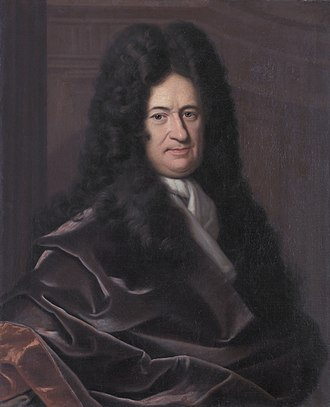
\includegraphics[width=0.45\textwidth]{figures/Gottfried_Wilhelm_Leibniz,_Bernhard_Christoph_Francke.jpg}
    \caption{Retrato de Gottfried Leibniz.\\Fuente: \href{https://es.wikipedia.org/wiki/Gottfried_Leibniz}{Wikipedia}}
    \label{fig:gottfried-leibniz}
\end{figure}

Aunque realmente la historia comienza en 1943 con la investigación de {Warren McCulloch} y {Walter Pitss}, publicaron el artículo \textit{A logical calculus of the ideas immanent in nervous activity} \cite{mcculloch1943logical}.
Dicho artículo creó distintas ramas de investigación (ordenadores digitales, inteligencia artificial, funcionamiento del perceptron).

\begin{figure}[H]
    \centering
    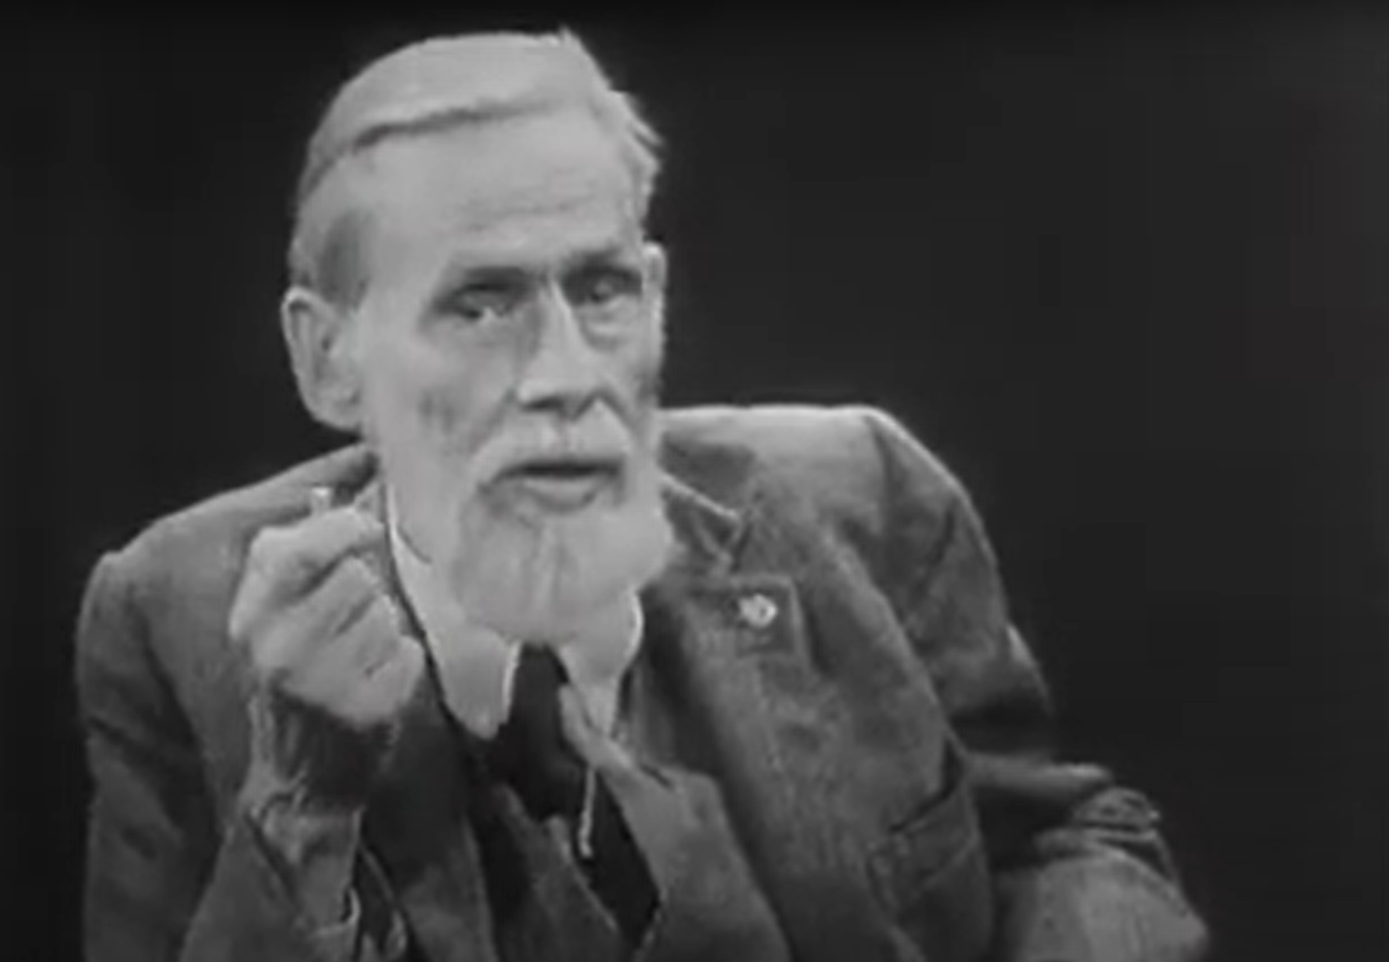
\includegraphics[width=0.65\textwidth]{figures/Warren Sturgis McCulloch Interview.png}
    \caption{Warren Sturgis McCulloch Interview.\\Fuente: \href{https://www.youtube.com/watch?v=8Wdz1Tj5084}{Entrevista en 1969}}
    \label{fig:Warren Sturgis McCulloch}
\end{figure}


En 1956 en la primera conferencia de inteligencia artificial organizada por la fundación {Rochester}, se reunen los investigadores fundadores de los conceptos actuales de la IA ({Minsky, McCarthy, Rochester, Shanon}), gran parte de la bibliografía se refiere a este punto como el origen y contacto de las redes neuronales artificiales.
En dicha conferencia (\textit{Nathaural Rochester}) presento el modelo de una red neuronal que fue el resultado de la investigación desarrollada por el equipo de investigación de IBM.

\begin{figure}[H]
    \centering
    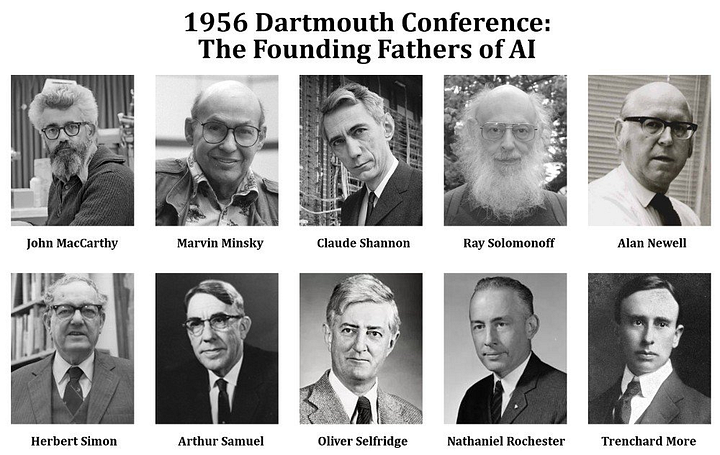
\includegraphics[width=0.75\textwidth]{figures/conferecia 1956 - 1689170718524.png}
    \caption{Los padres de la inteligencia artificial.\\Fuente: \href{https://www.linkedin.com/pulse/first-ever-ai-conference-tracing-evolution-history-ofai-nicky-verd}{Linkedin}}
    \label{fig:conferencia-1956}
\end{figure}

En 1957 se presenta el ``\textit{Perceptron}'' por {Frank Rosenblatt}, dicho elemento es un sistema clasificador de patrones, además contaba con la capacidad de aprender, de ser robusto matemáticamente y poder adaptarse si algún componente se dañaba.

\begin{figure}[H]
    \centering
    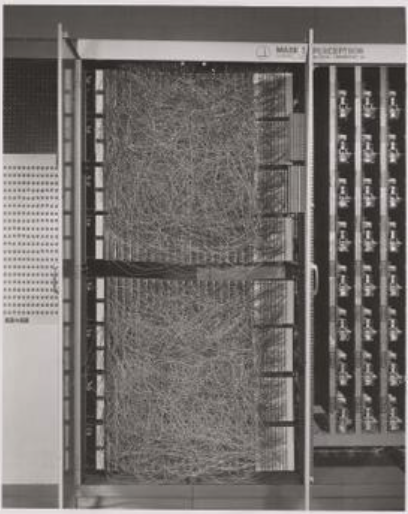
\includegraphics[width=0.4\textwidth]{figures/perceptron.png}
    \caption{Mark I Perceptron.\\Fuente: \href{https://en.wikipedia.org/wiki/Perceptron}{Wikipedia}}
    \label{fig:perceptron}
\end{figure}

El \textit{Perceptron} fue diseñado originalmente para el reconocimiento óptico usando un sistema de 400 fotocélulas en rejilla.
Posteriormente se describió el problema de no-linealidad que presentaban los perceptrones (Problema XOR) \cite{cuevastello2018apuntes}.

De 1959 a 1960 {Bernard Widrow} y {Ted Hoff} desarollaron ``Adaline'' y ``Madaline'' \cite{widrow1960adaptive} que resolvía el problema de la no-linealidad y que tenía aplicación en el reconocimiento de voz, series temporales, caracteres, etc.

Posteriormente el \textit{MIT} realizo una investigación matemática muy crítica de todos los problemas que presentaba el \textit{Perceptron} llegando a la conclusión que tenían grandes problemas que no podrían ser resueltos, por lo que en la próxima década (años 60) se redujo drásticamente las investigaciones sobre el campo de las redes neuronales.
Esto llevo a uno de los famosos inviernos de la inteligencia artificial (1974 - 1980).

\begin{figure}[H]
    \centering
    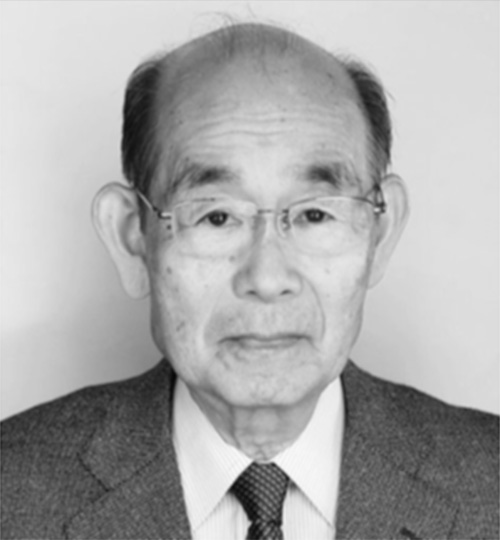
\includegraphics[width=0.25\textwidth]{figures/Kunihiko Fukushima.jpg}
    \caption{Kunihiko Fukushima.\\Fuente: \href{https://www.ieice.org/eng/about_ieice/new_honorary_members_award_winners/2017/meiyo_05e.html}{IEICE}}
    \label{fig:kunihiko-fukushima}
\end{figure}

Durante la década de los 70 se hacen aportes a la teoría \textit{Hebbiana}, se aportan logros en al análisis y descripción de reglas adaptativas, además de otros aportes al principio de aprendizaje competitivo.
En 1979 presentó {Kunihiko Fukushima} la primera red neuronal \acrshort{cnn}, la llamó Neocognitron \cite{fukushima1979neural}, dicho trabajo en un futuro se mejoraría con técnicas de \gls{BP-NN}.

En la década de los 80 se realizaron aportes como el algoritmo de \gls{BP-NN} que surgio del artículo de {Hopfield} \cite{hopfield1982neural}, esto despertó la curiosidad de muchos investigadores a volver al campo de las redes neuronales.
Se realizaron aportes como las redes \acrshort{gnn}.
La investigación continuó con {Stephen Grossberg} que realizo aportes derivados de estudios fisiológicos de cómo funcionaban las neuronas y la plasticidad, lo que permitió la creación de reglas y postulados, esto se ve en los trabajos de las redes \acrshort{art-nn} \cite{grossberg1987competitive}.
La investigación de {Hopfield} basada en el trabajo de {Stephen Grossberg} creo un sistema computacional neuronal interconectado que tiende a un mínimo de energía.
En 1985 {David E. Rumelhart} basandose en la investigación realizada por {Paul Werbos} \cite{etde_5080493} realizo un análisis experimental del algoritmo \gls{BP-NN} y su aplicación en redes \acrshort{fnn} \cite{rumelhart1985learning}.

{Yann LeCun} junto a su equipo, en 1989 crearon la primera aplicación \acrshort{cnn} con técnicas \acrshort{bp} dicha aplicación podía reconocer números a partir de imágenes.

\begin{figure}[H]
    \centering
    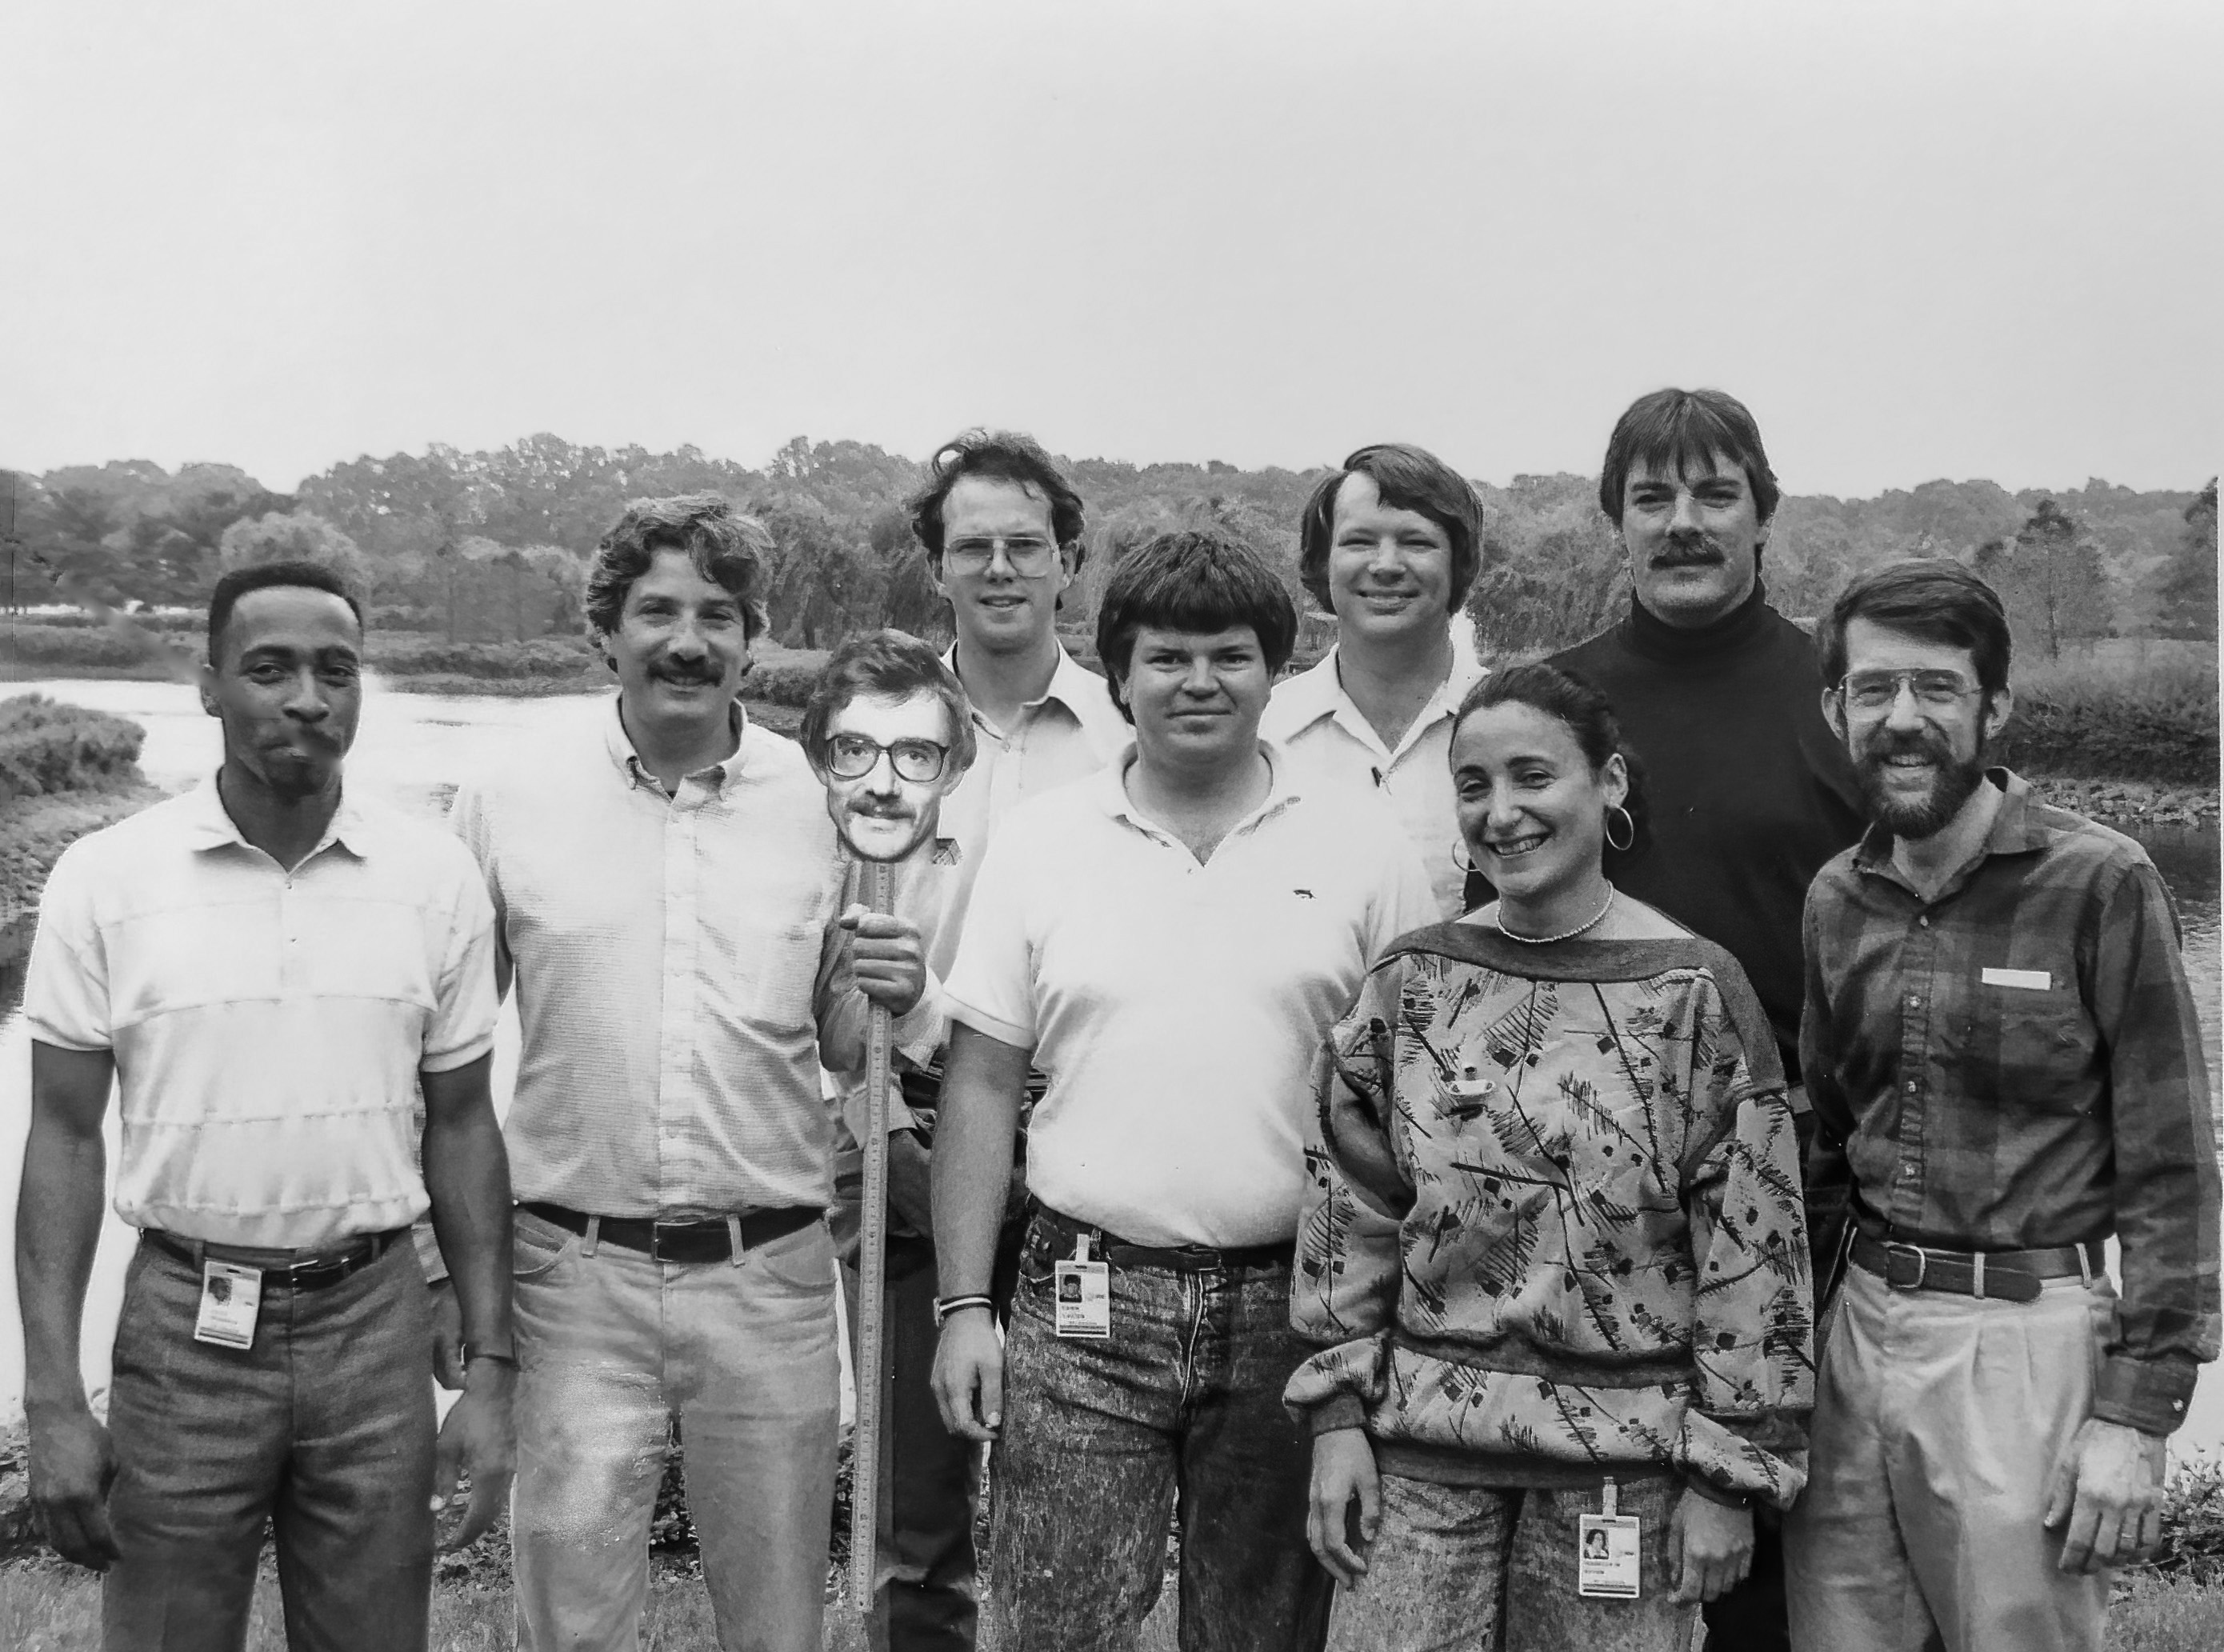
\includegraphics[width=0.65\textwidth]{figures/yann-lecun - EyIwmEDW8AIQs1C.jpeg}
    \caption{Adaptive Systems Research Department at Bell Labs 1989.\\Fuente: \href{https://twitter.com/ylecun/status/1378718317695934465}{Twitter Yann Lecun}}
    \label{fig:adaptive-systems-research-department-at-bell-labs}
\end{figure}

En la década de los 90 se presentaron múltiples investigaciones y muchos avances en el campo, uno de los más importantes fue la presentación de la primera \acrshort{gan} como una curiosidad, ya que se presentó como un duelo entre dos redes neuronales, en un principio fue un generador probabilístico y un predictor con el objetivo de maximizar la pérdida de cada uno en un juego \textit{minimax}.

En 1991 se presentó el trabajo \textit{Predictability Minimization} \cite{urgen1991learning} dichas técnicas sirvieron de inspiración para el aprendizaje por refuerzo,
En marzo de 1991 se hizo una aproximación a los \textit{transformers} con auto atención, lograron separar el conocimiento del control como una máquina clásica, pero de una forma completamente neuronal, además de gestionar actualizaciones de los pesos de forma muy rápida y eficiente.

Durante la década de 1990 las redes neuronales tendían a ser muy sencillas, con pocas capas y no muy complejas por las limitaciones técnicas de la época.
Por lo que muchos investigadores propusieron soluciones similares a las redes \acrshort{rnn} que permitían una retroalimentación, además de aceptar secuencias de información arbitraria.
Otros propusieron soluciones como la jerarquía de \acrshort{rnn} autosupervisada que aprende representaciones en distintos niveles de abstracción.
Comienzan a proponerse redes similares a las que en un futuro se llamarían \acrshort{dbn} como un método no supervisado para \acrshort{fnn}.

En junio de 1991 {Sepp Hochreiter} Figura \ref{fig:sepp-hochreiter} implemento el primer compresor de redes neuronales, además demostró uno de los principales problemas de las \acrshort{nn} el llamado problema del desvanecimiento o explosión del gradiente \ref{gradient-descent} que hacía que el aprendizaje fallará.
Un análisis posterior condujo a los investigadores a una primera aproximación \acrshort{lstm}, aunque no sería hasta 1997 con la revisión por pares y publicación del artículo \textit{Long short-term memory} \cite{hochreiter1997long} que se solucionaría parcialmente el problema.

\begin{figure}[H]
    \centering
    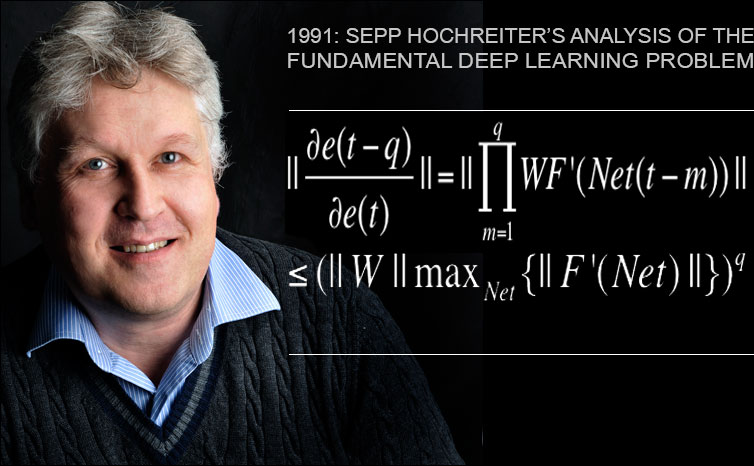
\includegraphics[width=0.65\textwidth]{figures/Sepp Hochreiter.jpg}
    \caption{Sepp Hochreiter.\\Fuente: \href{https://people.idsia.ch/~juergen/fundamentaldeeplearningproblem.html}{IDSIA}}
    \label{fig:sepp-hochreiter}
\end{figure}

Más adelante en el 2014 {Goodfellow} Figura \ref{fig:gan-ian-goodfellow} presento la primera red neuronal \acrshort{gan} pura para la generación de imágenes mediante el enfrentamiento de una red neuronal generativa contra una red neuronal discriminante entrenadas con el mismo conjunto de datos \cite{goodfellow2014generative}.
Durante los próximos años se realizaron muchos aportes a las redes neuronales generativas, principalmente de paralelización de los cálculos, técnicas de estabilización, generación condiciona, arquitecturas más eficientes, funciones de pérdidas más adecuadas, aplicaciones específicas (cambiar el estilo de pintura), redes apiladas, etc.
Fruto de todo ello {NVIDIA} en 2018 presento \gls{StyleGAN} \cite{karras2019stylebased} aunque publicaron el código en 2019 con fuertes mejoras.

\begin{figure}[H]
    \centering
    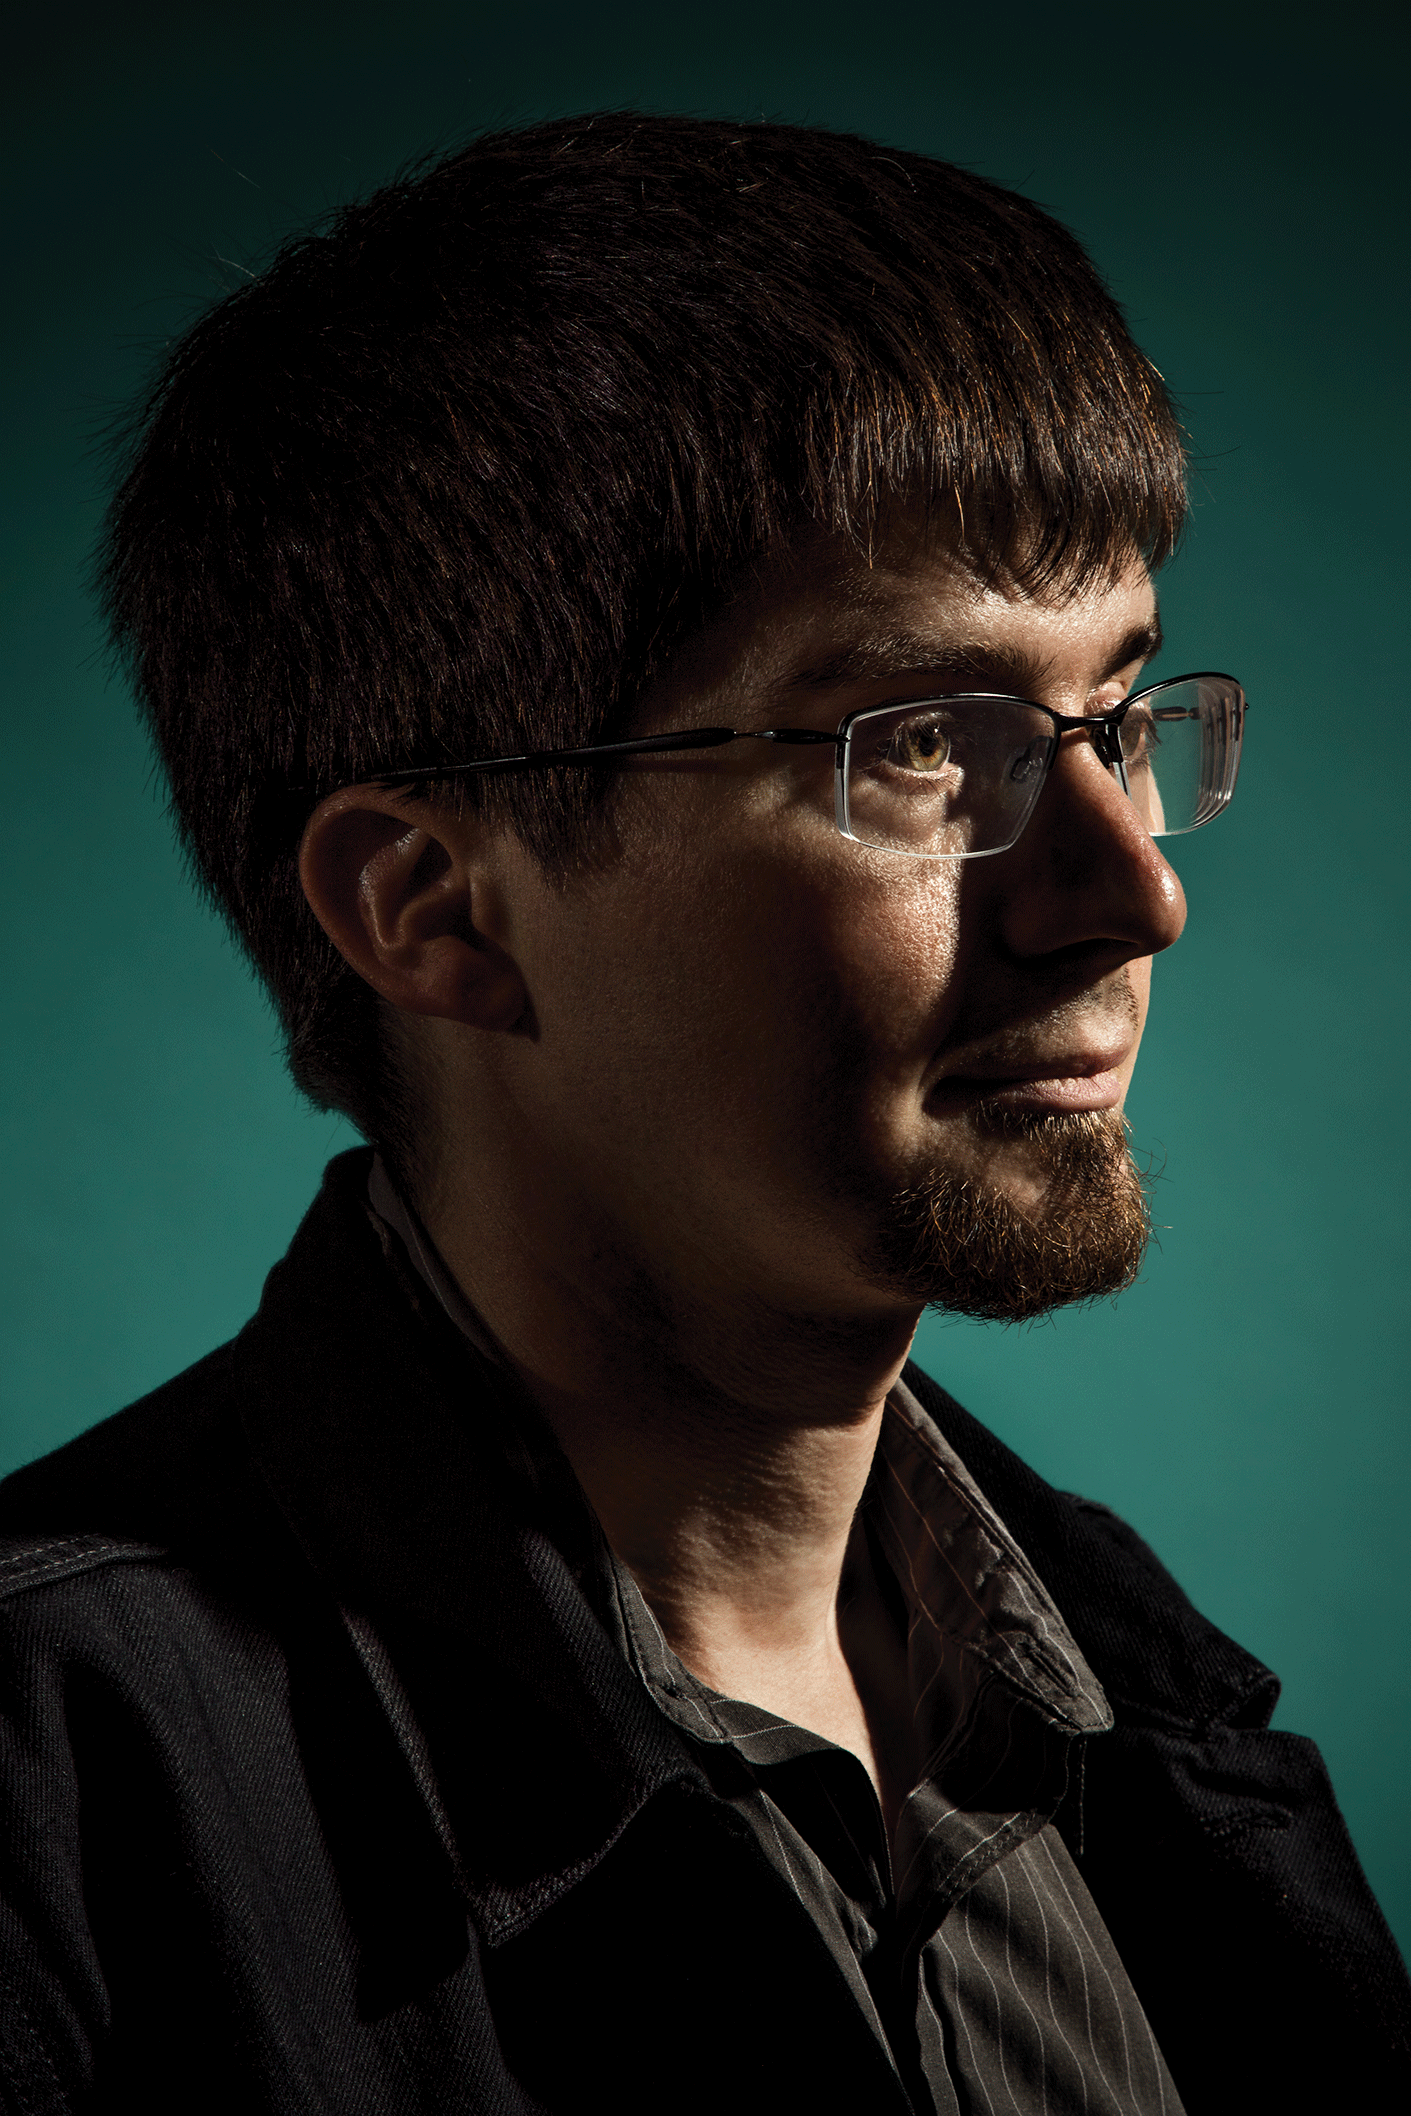
\includegraphics[width=0.2\textwidth]{figures/gan-goodfellow.png}
    \caption{Ian Goodfellow.\\Fuente: \href{https://www.technologyreview.es/s/10016/el-senor-de-las-gan-el-hombre-que-dio-imaginacion-las-maquinas}{MIT Technology Review}}
    \label{fig:gan-ian-goodfellow}
\end{figure}
% endregion


\section{Estado del arte}
\label{ch:2:section:state-of-the-art}

% region Teoría
\subsection{La ciencia de datos}
La ciencia de datos (\textit{Data Science}) es el estudio de los datos con el objetivo de extraer información útil, se usa principalmente para dar información útil a empresas. Es un campo multidisciplinar, ya que combina campos de las matemáticas, estadistica e inteligencia artificial para analizar grandes cantidades de datos. Esto tiene como objetivo responder a las siguientes cuestiones: \textit{¿Qué paso?, ¿Por qué pasó?, ¿Qué pasará? o ¿Qué se puede hacer con los resultados?} \cite{aws-data-science}

La ciencia de datos analiza los datos de distintas formas.

\begin{enumerate}
    \item \textbf{Análisis descriptivo}: examina datos con visualizaciones (gráficos, tablas) para entender eventos pasados o actuales.
    \item \textbf{Análisis de diagnóstico}: profundiza en los datos para entender las razones detrás del evento. Emplea técnicas cómo descubrimiento de datos o correlaciones.
    \item \textbf{Análisis predictivo}: utiliza datos históricos y técnicas como machine learning para hacer predicciones precisas sobre patrones futuros.
    \item \textbf{Análisis prescriptivo}: busca la mejor respuesta para un resultado esperado. Utiliza técnicas como simulación y redes neuronales para recomendar el mejor curso de acción entre varias alternativas.
\end{enumerate}


\subsection{La mineria de datos}
% Fases de la extraccón del conocimiento 
% Dentro del KDD está la {Mineria de datos}

La minería de datos, es una técnica asistida por computadora, procesa grandes conjuntos de datos para descubrir patrones y relaciones ocultas. Este conocimiento resultante se aplica en la resolución de problemas, análisis de decisiones empresariales, etc. Esta técnica tiene distintas fases para procesar y extraer información útil.

\begin{enumerate}
    \item Comprender, identificar y definir el alcance del proyecto.
    \item Comprender los datos.
    \item Depurar datos (limpiar, integrar y dar formato).
    \item Modelar datos.
    \item Evaluar los resultados.
    \item Implementar resultados.
\end{enumerate}

La mineria de datos es distinta en función de los datos y el objetivo, la mayoria del estado del arte segmenta la mineria en tres tipos, mineria de procesos, mineria de textos y mineria predictiva.

El Descubrimiento de Conocimientos en Bases de Datos \gls{KDD} es un proceso que utiliza algoritmos de minería de datos para explorar y extraer conocimientos útiles de grandes bases de datos. Con el avance tecnológico, se emplean técnicas de inteligencia artificial para este propósito, con el objetivo final de obtener conocimiento de alto nivel a partir de datos de bajo nivel. La Figura \ref{fig:kdd} esquematiza el proceso general del \textit{KDD}.

\begin{figure}[H]
    \centering
    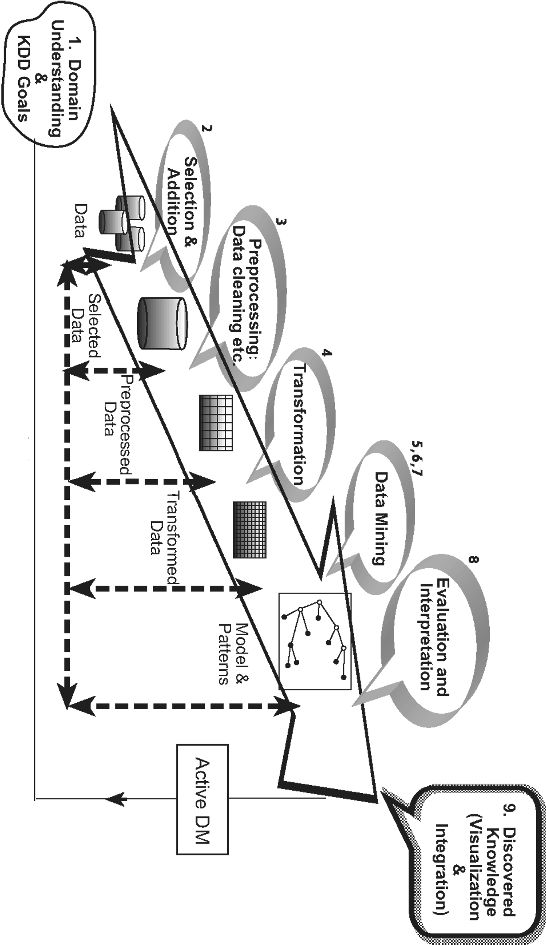
\includegraphics[angle=90,width=0.8\textwidth]{figures/chapter02/KDD.jpg}
    \caption{El proceso de descubrimiento de conocimiento en bases de datos.\\Fuente: Sección \textit{Introduction to Knowledge Discovery and Data Mining} \cite{rokach2010data}}
    \label{fig:kdd}
\end{figure}


\begin{enumerate}
    \item \textbf{Comprensión del Dominio de Aplicación}: se debe comprender los datos que se tratan y el campo de obtención con el objetivo de preparar los datos.
    \item \textbf{Selección y Creación de Conjunto de Datos}: se han de seleccionar los datos relevates (Selección de características).
    \item \textbf{Preprocesamiento y Limpieza de Datos}: se han de eliminar las características no relevantes, datos perturbados, entradas incoherentes o tratar datos faltantes, etc. con el objetivo de obtener datos más limpio.
    \item \textbf{Transformación de Datos}: se deben tratar los datos, reduciendo la dimensionalidad, filtración, descomponiendo, etc. para que sea más sencillo el consumo de estos datos por una aplicación.
    \item \textbf{Elección de Tarea de Minería de Datos}: en función de los datos y del objetivo deberemos realizar una tarea (clasificación, regresión o agrupación), ya que en la mineria de datos hay dos objetivos principales, \textbf{predicción} y \textbf{descripción}.
    \item \textbf{Elección del Algoritmo de Minería de Datos}: deberemos elegir entre los distintos algoritmos que se usan en la mineria de datos, si buscamos precisión podemos usar redes neuronales, si buscamos explicabilidad podemos usar arboles de decisión.
    \item \textbf{Implementación del Algoritmo de Minería de Datos}: emplearemos el algoritmo seleccionado ajustando las parámetros para que nos de el mejor resultado.
    \item \textbf{Evaluación de Patrones Minados}: debemos interpretar los resultados (reglas, confiabilidad, etc) si no cumplen los objetivos que se buscaban en el primer paso deberemos reajustar toda la metodologia, desde ajustar la selección de características a la interpretación o compresibilidad del modelo.
    \item \textbf{Utilización del Conocimiento Descubierto}: por último debemos incorporar el conocimiento a los sistemas de toma de decisiones, este es el paso más importante, ya que con el podemos medir los efectos del conocimiento obtenido. Puede suceder que una vez implementado el modelo en sistema de producción pierda eficiencia si las condiciones reales son distintas a las de la creación del modelo.
\end{enumerate}


\begin{figure}[H]
    \centering
    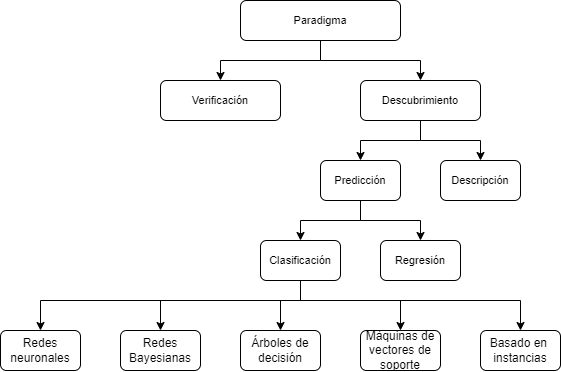
\includegraphics[width=\textwidth]{figures/chapter02/data-mining-taxonomy.drawio.png}
    \caption{Taxonomía de minería de datos.\\Fuente: Elaboración propia, inspirado en la sección \textit{Introduction to Knowledge Discovery and Data Mining} \cite{maimon2005data}}
    \label{fig:data-mining-taxonomy}
\end{figure}

La mineria de datos puede estár orientada a la verificación o al descubrimiento de patrones, se debe automatizar su identificación, puediendo usar un efoque predictictivo o descriptivo. Para el descubrimiento se usa el aprendijaze inductivo, mientras que en la verificación se ha de evaluar la hipótesis externas usando métodos estádisticos clásicos. La terminología clásica del aprendizaje automatico está clasificado en supervisado (clasificación y regresión) y no supervisado (agrupamiento), aunque existen muchos más términos en la terminología moderna esto podemos analizarlo más en profundidad en el libro \textit{Data Mining and Knowledge Discovery Handbook} \cite{maimon2005data}.


\subsection{Aprendizaje automático - \textit{Machine Learning}}

El \textit{machine learning} es la ciencia o rama de la inteligencia artificial que desarrolla, modelos estadisticos, desarrolla algoritmos que generalizan comportamientos y reconocen patrones. Es decir hace posible el aprendijaze autónomo de las máquinas para realizar tareas sin la necesidad programar las instrucciones explícitamente. El \textit{machine learning} busca procesar grandes cantidades de datos e identificar patrones de datos de forma automática.

\begin{figure}[H]
    \centering
    \centerline{\includesvg[width=0.75\linewidth]{figures/chapter02/machine-learning-rules.drawio.svg}}
    \caption{El \textit{Machine Learning} como paradigma de programación.\newline{}Fuente: Elaboración propia.}
    \label{fig:machine-learning-rules}
\end{figure}

Como podemos ver en la figura \ref{fig:machine-learning-rules} el paradigma clásico se necesitaba conocer el dominio de los datos y las reglas en profundidad y programar los descriptores de forma manual para procesar los datos. En el paradigma del \textit{machine learning} permite extraer esas reglas y patrones para procesar nuevos datos a partir de respuestas que conociamos previamente, estas respuestas previas deben ser extraidas o validadas por expertos.

Una clásificación de las tareas del \textit{machine learning} lo podemos ver en la figura \ref{fig:machine-learning}, esta clasificación está dividida en función de como se realiza el aprendijaze del modelo.

\begin{figure}[H]
    \centering
    \centerline{\includesvg[width=1\linewidth]{figures/chapter02/machine-learning.drawio.svg}}
    \caption{Clasificación de los algoritmos de aprendijaze automático.\\Fuente: Elaboración propia.}
    \label{fig:machine-learning}
\end{figure}

El \textit{machine learning} puede trabajar con datos estructurados y no estructurados aunque estos últimos requieren un procesamiento previo para adapatarlos en un formato estructurado.



\subsection{Aprendizaje profundo - \textit{Deep Learning}}
% TODO: Explicar el Deep Learning https://idus.us.es/bitstream/handle/11441/90004/Centeno%20Franco%20Alba%20TFG.pdf

El \textit{deep learning} es una subrama del \textit{machine learning} que usa redes neuronales artificiales para analizar datos no lineales, estas redes imitan el comportamiento del cerebro humano, para esto suelen contar con arquitecturas complejas.

El \textit{deep learning} se distingue del \textit{machine learning} por los tipos de datos con los que puede trabajar y por los métodos con los que hace que los modelos aprendan.

Otra de las carácteristicas que diferencia al \textit{deep learning} del \textit{machine learning} es que elimina parte del procesamiento previo de datos, ya que sus algoritmos puede ingerir y procesar datos no estructurados.


%  ==============================================================================
%  ==============================================================================
%  ==============================================================================

\subsection{Redes neuronales - \textit{Neuronal Networks}}
% TODO: \cite{ibm-deep-learning}
% Explicar uso de multiples neuronas artificiales para crear capas y luego redes
El \textit{deep learning} emplea principalmente redes neuronales para reconocer, clasificar y describir con precisión patrones de datos. Estas redes están inspiradas en el funcionamiento del cerebro humano.  \cite{ibm-deep-learning}

Las redes neuronales es un conjunto de neuronas artificiales que están organizadas generalmente por capas. Estas redes tienen una capa de entrada, una capa de salida y multiples capas ocultas con distintas funciones de activación que ponderan los pesos de cada neurona.

Las redes neuronales cuentan con formas muy variadas de componer las capas, a esto se le denomina \textbf{topologia de red neuronal}, en función del objetivo que se busque, la topologia será muy distinta.

\subsubsection{Elementos de una neurona artificial}

Como se ha comentado previamente las neuronas artificiales están inspiradas en las neuronas biologicas del cerebro humanos, fueron los investigadores \textit{McCulloch} y \textit{Pitts} \cite{mcculloch1943logical} los que sentaron las bases de lo que es una neurona artificial, demostrando que su modelo de red neuronal podía realizar cálculos que se correspondían con la lógica proposicional.

\begin{figure}[H]
    \centering
    \centerline{\includesvg[width=1\linewidth]{figures/chapter02/artificial-neuron.drawio.svg}}
    \caption{Partes de una neurona artificial bioinspirada en una neurona biológica.\\Fuente: Elaboración propia}
    \label{fig:artificial-neuron}
\end{figure}

En la Figura \ref{fig:artificial-neuron} podemos ver las distintas partes de una única neurona artificial y sus partes equivalentes con una neurona biológica. El axón opera como la entrada de información a la neurona,



% Perceptron
%% LTU 

% Perceptron simple: %% solo dos capas, la red es unidireccional, la primera capa no realiza calculos, solo consume los datos de entrada, la segunda capa unicamente aplica una f. de activación de paso o signo 
% Perceptrón múltiple

\subsubsection{Funcionamiento de una red neuronal \label{neural-network}}

Las redes neuronales profundas tienen multitud de capas con nodos interconectados, cada capa sobre la capa anterior con el objetivo de optimizar la precisión de una predición o clasificación. A esta progresión de calculos se le denomina ``propagación hacia delante''.

El proceso de ``propagación inversa'' es el encargado de calcular errores de precisión, ajustar sesgos y ponderaciones usando algoritmos como el descenso de gradiente \ref{gradient-descent}.

La capa de entrada es por donde el modelo ingiere los datos, y la capa de salida es donde el modelo responderá con la predicción o clasificación.

\begin{figure}[H]
    \centering
    \centerline{\includesvg[width=1\linewidth]{figures/chapter02/neuronal-network.drawio.svg}}
    \caption{Red neuronal artificial.\\Fuente: Elaboración propia}
    \label{fig:artificial-neuronal-network}
\end{figure}

En la Figura \ref{fig:artificial-neuronal-network} podemos ver una arquitectura simple de una red neuronal que cuenta con la capa de entrada, la capa de salida y dos capas ocultas.

El vector de entrada $X = (x_{1}, x_{2}, ..., x_{n})$ será la información suministrada a nuestro red a través de la capa de entrada, este vector será de tamaño $n$.


\begin{figure}[H]
    \centering
    \centerline{\includesvg[width=1\linewidth]{figures/equations/Notation.drawio.svg}}
    \caption{Calculo de los pesos de la red neuronal artificial\\Fuente: Elaboración propia}
    \label{fig:notation}
\end{figure}

% region: el descenso de gradiente
\subsubsection{El descenso de gradiente \label{gradient-descent}}
% TODO: explicar el descenso de gradiente

El problema de desvanecimiento y explosión de gradiente


% endregion


% Multicapa
% Capas
% Funciones de optimización
% Funciones de activación
% Funciones de perdida
% Topologias

\subsubsection{Tipos de capas}


\begin{itemize}
    \item \textbf{Capa de entrada}:
    \item \textbf{Capas ocultas}:
    \item \textbf{Capa de salida}:
\end{itemize}





\paragraph*{\textit{Non-linear Activations (weighted sum, nonlinearity)} \cite{pytorch2024github}}

\begin{enumerate}
    \item \textbf{ReLu}:
    \item[] \begin{equation} \varphi(x) = \operatorname*{max}(0,x) \end{equation}
        \begin{figure}[H]
            \centering
            \includegraphics[width=0.5\textwidth]{figures/equations/ReLu.png}
            \caption{Función de activación ReLu\\Fuente: \href{https://pytorch.org/docs/stable/generated/torch.nn.ReLu.html}{Pytorch torch.nn.ReLu}}
            \label{fig:torch.nn.ReLu}
        \end{figure}

    \item \textbf{Sigmoid}:
    \item[] \begin{equation} \varphi(x) = \frac{1}{1+e^{-x}} \end{equation}
        \begin{figure}[H]
            \centering
            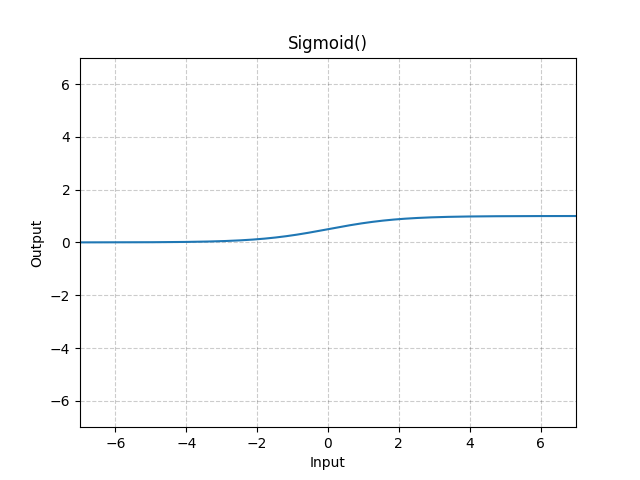
\includegraphics[width=0.5\textwidth]{figures/equations/Sigmoid.png}
            \caption{Función de activación Sigmoid\\Fuente: \href{https://pytorch.org/docs/stable/generated/torch.nn.Sigmoid.html}{Pytorch torch.nn.Sigmoid}}
            \label{fig:torch.nn.Sigmoid}
        \end{figure}

    \item \textbf{Softplus}:
    \item[] \begin{equation} \varphi(x) = \frac{1}{\beta} \operatorname*{log}(1+e^{\beta x}) \end{equation}
        \begin{figure}[H]
            \centering
            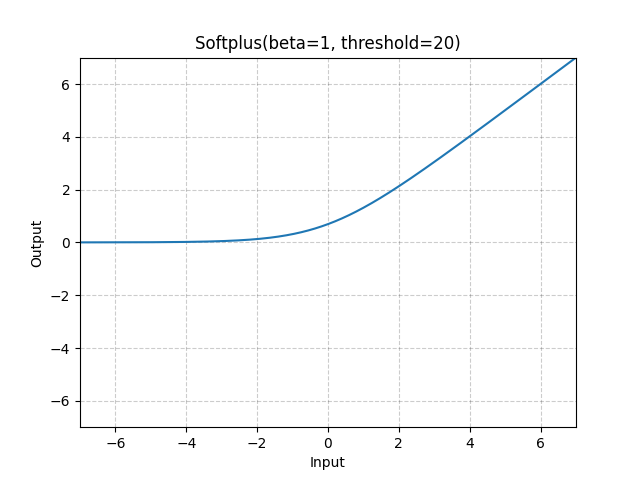
\includegraphics[width=0.5\textwidth]{figures/equations/Softplus.png}
            \caption{Función de activación Softplus\\Fuente: \href{https://pytorch.org/docs/stable/generated/torch.nn.Softplus.html}{Pytorch torch.nn.Softplus}}
            \label{fig:torch.nn.Softplus}
        \end{figure}

    \item \textbf{Tanh}: text.
    \item[] \begin{equation} \varphi(x) = \frac{e^{x}-e^{-x}}{e^{x}+e^{-x}} \end{equation}
        \begin{figure}[H]
            \centering
            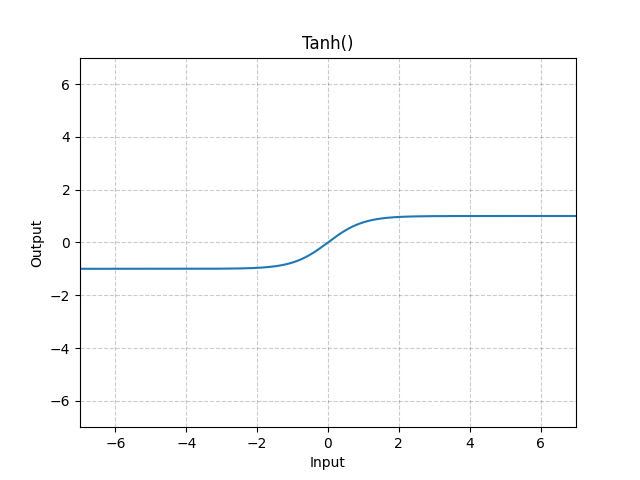
\includegraphics[width=0.5\textwidth]{figures/equations/Tanh.png}
            \caption{Función de activación Tanh\\Fuente: \href{https://pytorch.org/docs/stable/generated/torch.nn.Tanh.html}{Pytorch torch.nn.Tanh}}
            \label{fig:torch.nn.Tanh}
        \end{figure}

    \item \textbf{SoftSign}:
    \item[] \begin{equation} \varphi(x) = \frac{x}{1+\lvert x \rvert} \end{equation}
        \begin{figure}[H]
            \centering
            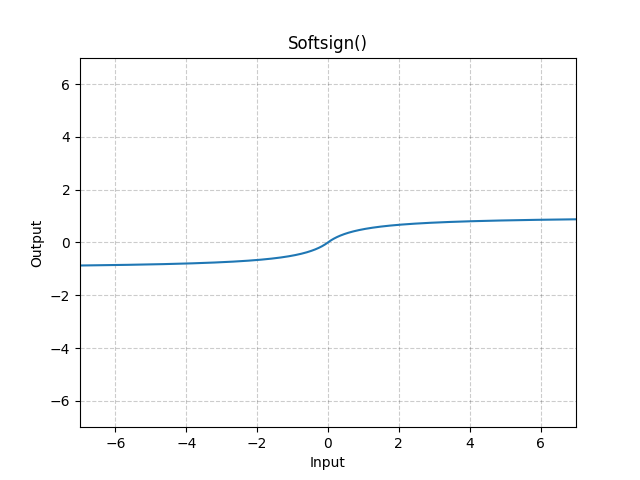
\includegraphics[width=0.5\textwidth]{figures/equations/Softsign.png}
            \caption{Función de activación Softsign\\Fuente: \href{https://pytorch.org/docs/stable/generated/torch.nn.Softsign.html}{Pytorch torch.nn.Softsign}}
            \label{fig:torch.nn.Softsign}
        \end{figure}
\end{enumerate}

\subparagraph{\textit{Non-linear Activations (other)} \cite{pytorch2024github}}
% TODO: explicar las funciones de activación no lineales más importantes

\begin{enumerate}
    \item \textbf{Softmax}: Aplica la función Softmax a un Tensor de entrada $n$-dimensional reescalándolos para que los elementos del Tensor de salida $n$-dimensional se encuentren en el rango [0,1]. \cite{pytorch2024github}
    \item[] \begin{equation} \varphi(x_{i}) = \frac{e^{x_{i}}}{\sum_{j}{e_{j}}} \end{equation}
\end{enumerate}



% region funciones de activación

% endregion

% region topologias
\subsubsection{Topologias de redes neuronales}
% TODO: explicar la existencia de distintas formas de aplicar las capas de neuronas artificiales y sus resultados

\begin{itemize}
    % \item[] 
    \item \textbf{Capas totalmente conectadas}
    \item \textbf{Capas localmente conectadas}
    \item \textbf{Capas convolucional}
    \item \textbf{Capas reductora \textit{pooling} y \textit{dropout}}
\end{itemize}


\begin{figure}[H]
    \centering
    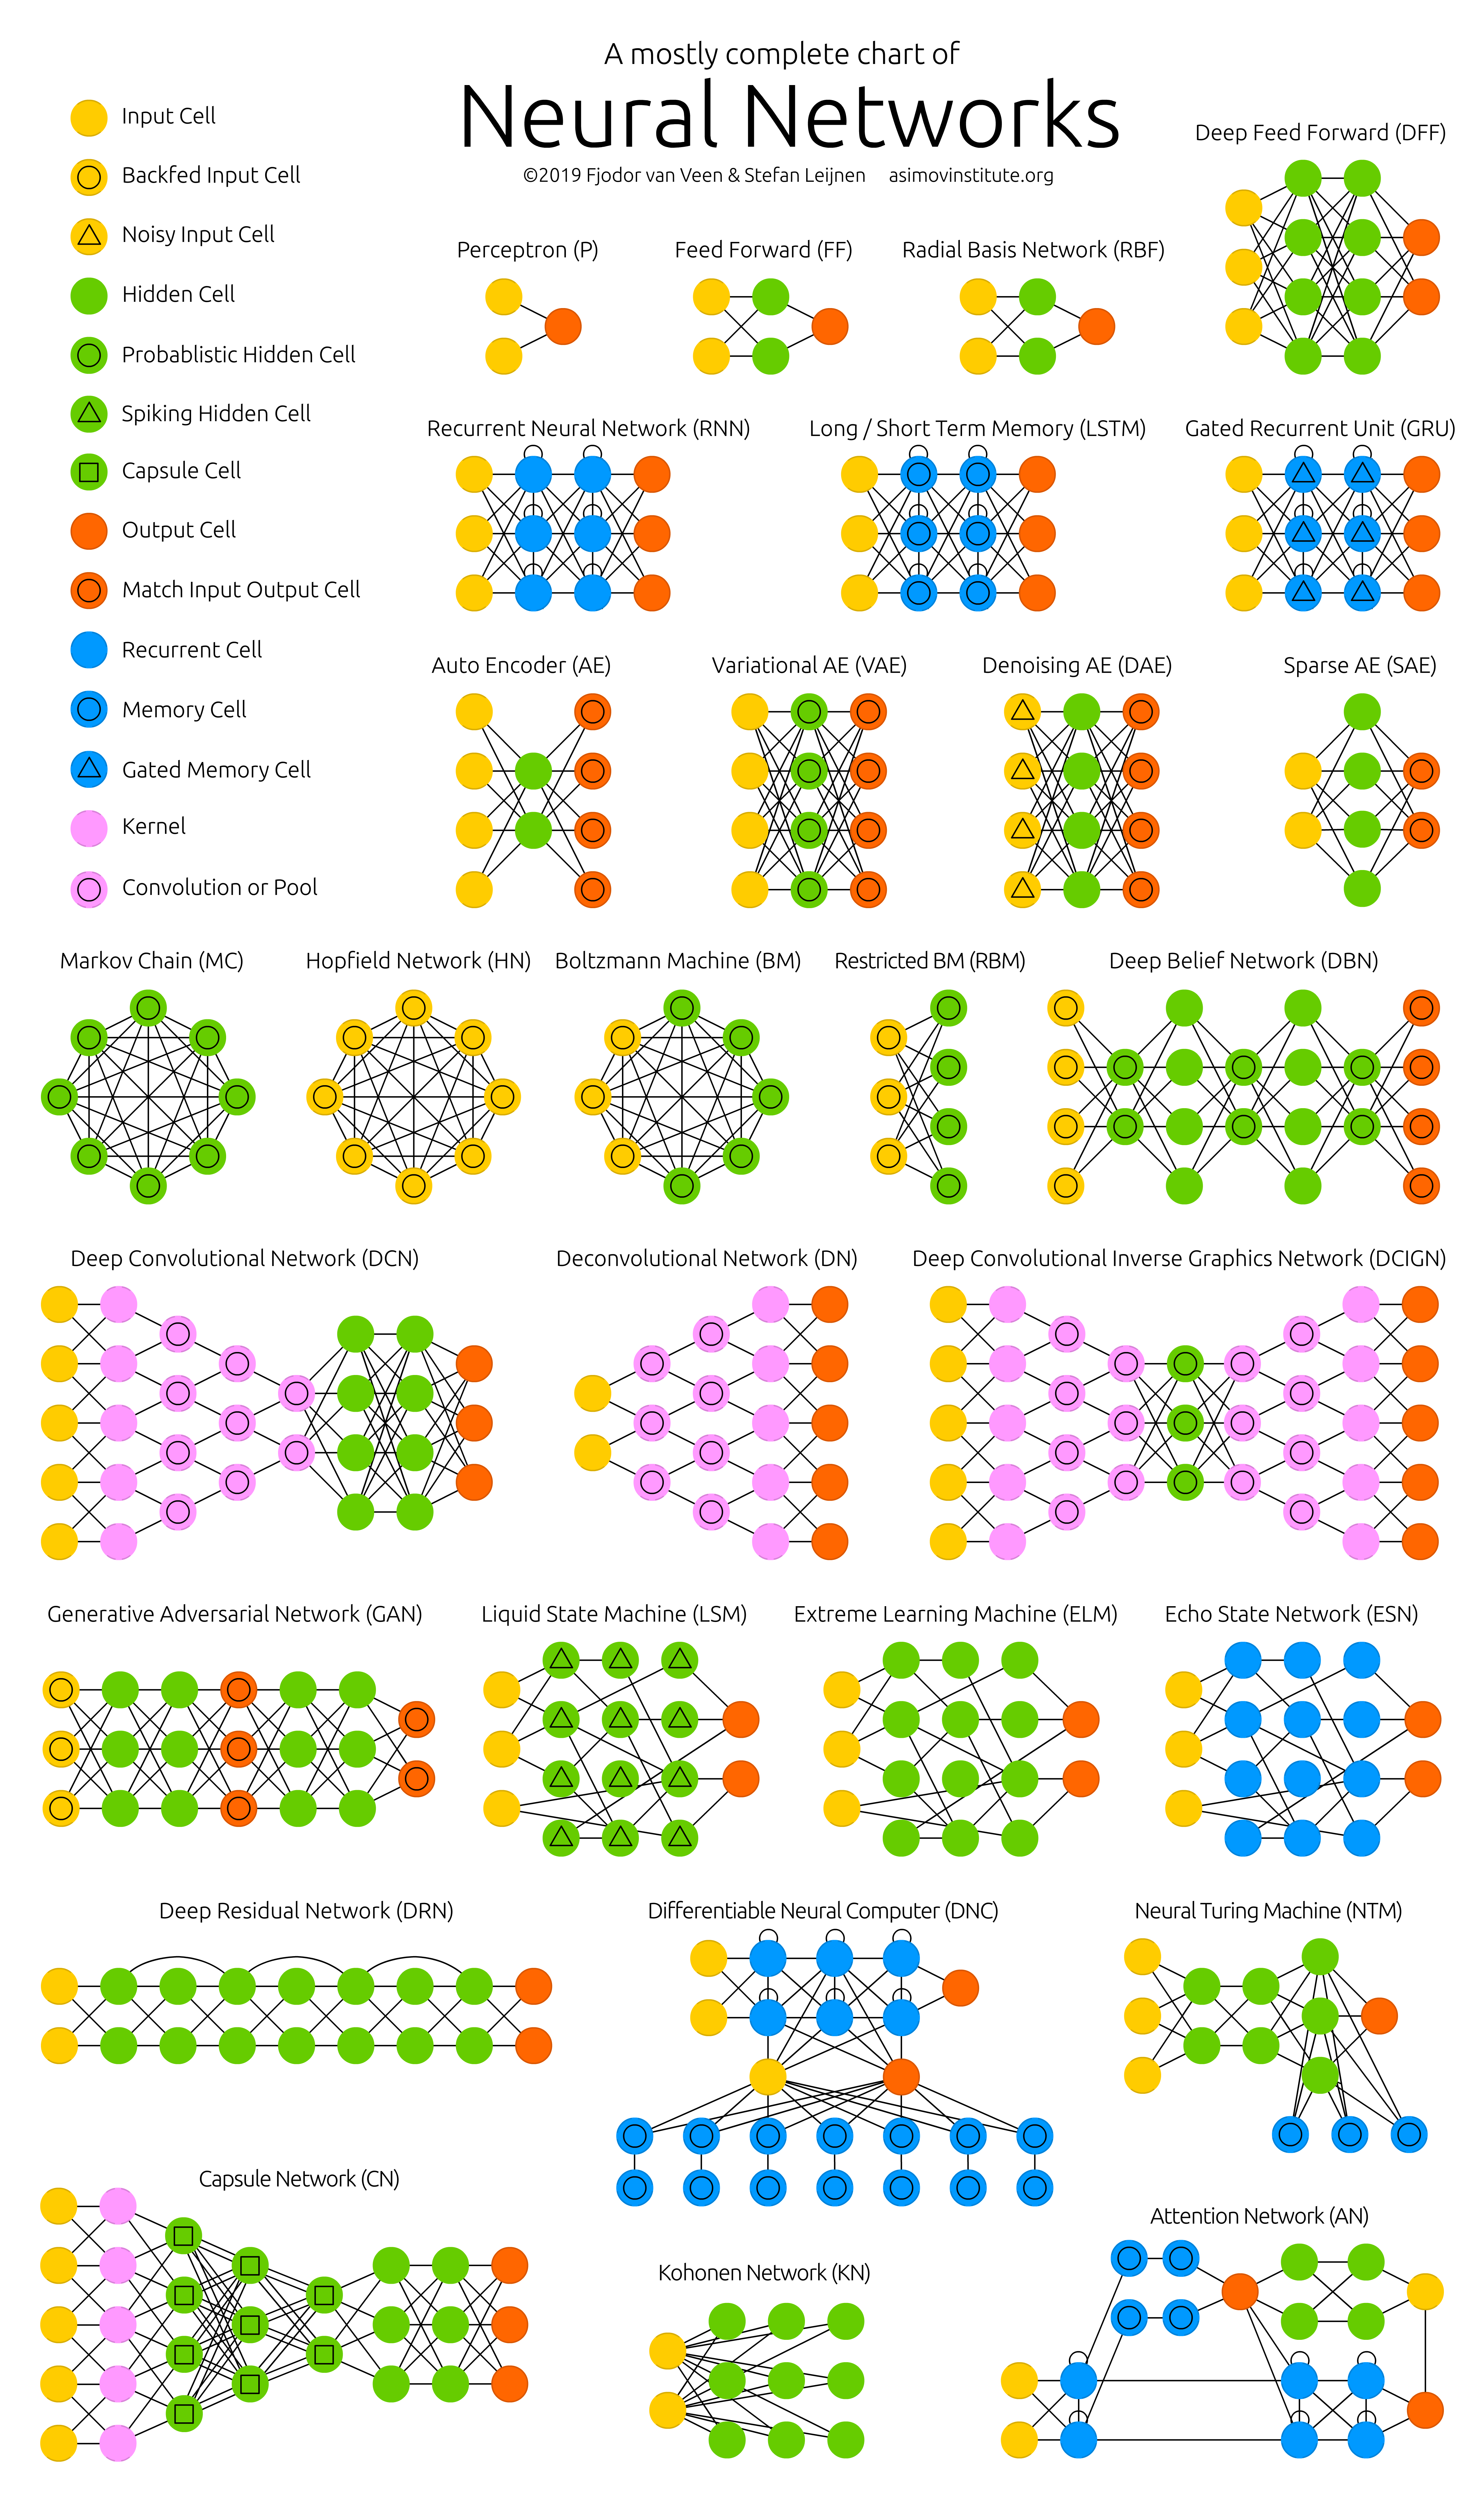
\includegraphics[width=0.8\textwidth]{figures/NeuralNetworkZo19High.png}
    \caption{Topologias de redes neuronales.\\Fuente: \href{https://www.asimovinstitute.org/neural-network-zoo/}{The neural network zoo}}
    \label{fig:NeuralNetworkZo19High}
\end{figure}
% endregion

% region AN
\subsection{Redes adversariales - \textit{Adversarial Networks}}
% TODO: 
% endregion

% region GAN
\subsection{Redes generativas adversariales - \textit{Generative Adversarial Networks (GAN)}}
% TODO:
\begin{figure}[H]
    \centering
    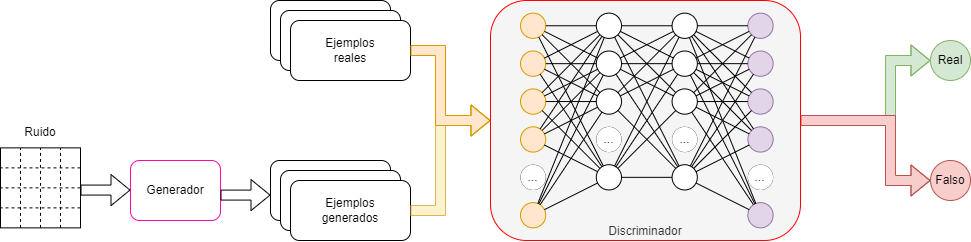
\includegraphics[width=1\textwidth]{figures/chapter02/GANs.drawio.png}
    \caption{Arquitectura de las redes neuronales generativas adversariales.\\Fuente: Elaboración propia.}
    \label{fig:gans-architecture}
\end{figure}
% endregion


% endregion

% region subsection La seguridad de las redes neuronales
\subsection{La seguridad de las redes neuronales}
\label{ch:2:section:state-of-the-art:computer-security-in-neural-networks}

El estado del arte de la seguridad es muy complejo por la constante evolución, las ciberamenazas están en constante evolución, los delincuentes informaticos adoptan nuevas técnicas y tácticas para eludir las medidas de seguridad tradicionales.

Dentro de la inteligencia artificial \gls{AI} encontramos el aprendizaje automático \gls{ML} y dentro el aprendijaze profundo \gls{DL}.
Para el desarrollo de este capítulo limitaremos el alcance del estado del arte de la seguridad informática a los campos relacionados con la inteligencia artificial.

\begin{figure}[H]
    \centering
    \centerline{\includesvg[width=1\columnwidth]{figures/chapter02/adversarial-threats.drawio.svg}}
    \caption{Amenazas adversariales.\\Fuente: Elaboración propia.}
    \label{fig:art-adversarial-threats}
\end{figure}

Como podemos observar en la figura \ref{fig:art-adversarial-threats} existen multitud de amenazas a redes neuronales.

% Eficiencia
% Invisivilidad
% Efectividad

\subsection{Amenazas en \textit{deep learning}}
% TODO
Existen cuatro formas de clasificar las amenazas de las redes neuronales en \gls{DL} en función de como se altera el comportamiento del modelo.

\subsubsection{Evasión}

Busca explotar las vulnerabilidades de la red neuronal para inducir errores en la capacidad de clasificar o de predecir. Se envia información con perturbaciones minimas que alteren notablemente la respuesta del modelo.

\begin{enumerate}
    \item \textbf{Caja blanca}: se conoce todo sobre el modelo, arquitectura, pesos, umbrales, formato de entreada de datos y salida, etc. \cite{learning-machine-learning-part-3-attacking}
    \item \textbf{Caja negra}: se desconoce el modelo, arquitectura, pesos, umbrales, pero se conoce el formato de entrada de datos y la respuesta del modelo. \cite{learning-machine-learning-part-3-attacking}
\end{enumerate}

\subsubsection{Envenenamiento}
% 

Los atacantes intentan manipular los datos de entrenamiento con el objetivo de influir en el resultado del aprendijaze del modelo, esto pueden hacerlo desde distintas etapas.

% $$ \sum_{rand}(x)=\left\{clip\left(x+\delta\right)|\delta\in[-5,5]^{H\times W\times3}\right\} $$

\begin{enumerate}
    \item \textit{Label Flipping Attacks} - Ataques de cambio de etiquetas:
    \item \textit{Clean Label Data Poisoning Attack} - Ataques de envenenamiento de datos de etiquetado limpio:
    \item \textit{Backdoor Attack} - Ataques de puerta trasera: los ataques de puerta trasera, ataques que contienen un disparador, estos se pueden clasificar en tres tipos de escenarios.
          \begin{enumerate}
              \item Aprendizaje d
              \item Aprendizaje por transferencia
              \item Aprendizaje federado
          \end{enumerate}
\end{enumerate}

\paragraph{Label Flipping Attacks}

\paragraph{Clean Label Data Poisoning Attack}


\subparagraph{Feature Collision Attack}
$$x_{p}={\underset{x}{\mathrm{argmin}}}||f\left(x\right)-f\left(x_{t}\right)||_{2}^{2}+\beta||x-x_{b}||_{2}^{2}\,,$$
% 


\subparagraph{Convex Polytope Attack and Bullseye Polytope Attack}

\paragraph{Backdoor Attack}


\subsubsection{Extracción}

Se busca extraer un funcionamiento interno equivalente de la red neuronal, se puede considerar un ataque de ingeniería inversa.

% 
\subsubsection{Inferencia}

\paragraph{Inferencia por Atributos}
\paragraph{Inferencia por Pertenencia}
\paragraph{Inversión de modelos}
\paragraph{Reconstrucción}

\subsection{Defensas contra los ataques en \textit{deep learning}}

\subsubsection{Pre procesamiento}
\subsubsection{Post procesamiento}
\subsubsection{Entrenamiento}
\subsubsection{Transformación}
\paragraph{Evasión}
\paragraph{Envenenamiento}
\subsubsection{Detector}
\paragraph{Evasión}
\paragraph{Envenenamiento}

\subsection{Metricas en los ataques adversariales}

\subsection{\textit{Red team} - \textit{Blue team} en redes neuronales}

Un buen simil entre la seguridad informática clásica y la seguridad en redes neuronales son los conceptos de equipos de ataque y defensa (``red team'' y ``blue team'').

\begin{figure}[H]
    \centering
    \centerline{\includesvg[width=1\columnwidth]{figures/chapter02/ART-for-red-and-blue-teams.drawio.svg}}
    \caption{Ataques y defensas en redes neuronales.\\Fuente: Elaboración propia.}
    \label{fig:art-for-red-and-blue-teams}
\end{figure}

La idea detrás del aprendizaje automático es la de poder predecir modelos predictivos, para ello se usan conjuntos de datos para el entrenamiento.

Los conjuntos de datos se han de procesar, ya que suelen contener mucho ruido, es decir, información muy poco valiosa, errónea o, por el contrario, una alta dimensionalidad de los datos que puede ser contraproducente por no poder reproducir esas medidas o por la poca información que aportan.

Los ataques al aprendizaje automático o profundo suelen estar dirigidos a las distintas etapas de creación y uso de un modelo.

\begin{itemize}
    \item Alteración de los datos de entrada.
    \item Alteración del proceso de aprendizaje.
    \item Extración de los datos de entrenamiento.
    \item Bloqueo del modelo.
\end{itemize}

Durante el transcurso del trabajo discutiremos los siguientes ataques y defensas previamente en la sección \nameref{ch:2:section:state-of-the-art:computer-security-in-neural-networks} que se pueden usar en los modelos.

\begin{itemize}
    \item Envenenamiento de datos.
    \item Puerta trasera.
    \item Extracción de datos
    \item Ingeniería inversa.
    \item Evasión.
\end{itemize}

Se puede ser categorizar la seguridad de los modelos con el modelado \gls{STRIDE} de microsoft\footnote{Modelado de amenazas de microsoft \href{https://learn.microsoft.com/es-es/azure/security/develop/threat-modeling-tool-threats}{Enlace}} o con la matriz \gls{MITRE}.

\begin{table}[H]
    \centering
    \small
    \def\arraystretch{1.5}
    \begin{tabular}{lp{10cm}}
        \toprule
        \textbf{Amenaza}    & \textbf{Tipo de ataque}                                           \\
        \midrule
        Corrupción de datos & Ataques de envenenamiento de datos, ataques de puerta trasera     \\
        Extracción de datos & Ataques de inferencia de membresía, ataques de ingeniería inversa \\
        Denegación          & Ataques de envenenamiento de datos                                \\
        \bottomrule
    \end{tabular}
    \caption{Amenazas STRIDE relacionadas con la seguridad de la IA}
    \label{tab:amenazas}
\end{table}

% endregion

% region subsection Las redes neuronales para la seguridad informática
\subsection{Las redes neuronales para la seguridad informática}
% TODO: aplicaciones reales de ciberseguridad que usan inteligencia artificial 


% endregion




\subsection{Normativa y estándares}
% https://eur-lex.europa.eu/resource.html?uri=cellar:e0649735-a372-11eb-9585-01aa75ed71a1.0008.02/DOC_1&format=PDF
% https://eur-lex.europa.eu/resource.html?uri=cellar:e0649735-a372-11eb-9585-01aa75ed71a1.0008.02/DOC_2&format=PDF

% Según la unión europea toda la seguridad es este apartado :ok: 
% (51) La ciberseguridad es fundamental para garantizar que los sistemas de IA resistan a las actuaciones de terceros maliciosos que, aprovechando las vulnerabilidades del sistema, traten de alterar su uso, conducta o funcionamiento o de poner en peligro sus propiedades de seguridad. Los ciberataques contra sistemas de IA pueden dirigirse contra elementos específicos de la IA, como los conjuntos de datos de entrenamiento (p. ej., contaminación de datos) o los modelos entrenados (p. ej., ataques adversarios), o aprovechar las vulnerabilidades de los elementos digitales del sistema de IA o la infraestructura de TIC subyacente. Por lo tanto, para asegurar un nivel de ciberseguridad adecuado a los riesgos, los proveedores de sistemas de IA de alto riesgo deben adoptar medidas adecuadas teniendo también en cuenta, cuando proceda, la infraestructura de TIC subyacente.









% https://www.youtube.com/@felipebravom



% Feb 1990: Generative Adversarial Networks / Curiosity Generative Adversarial Networks (GANs) have become very popular.[MOST] They were first published in 1990 in Munich under the moniker Artificial Curiosity. [AC90-20][GAN1] Two dueling NNs (a probabilistic generator and a predictor) are trying to maximize each other's loss in a minimax game.[AC](Sec. 1) The generator (called the controller) generates probabilistic outputs (using stochastic units[AC90] like in the much later StyleGANs[GAN2]). The predictor (called the world model) sees the outputs of the controller and predicts environmental reactions to them. Using gradient descent, the predictor NN minimizes its error, while the generator NN tries to make outputs that maximize this error: one net's loss is the other net's gain.[AC90] (The world model can also be used for continual online action planning.[AC90][PLAN2-3][PLAN])

% 4 years before a 2014 paper on GANs,[GAN1] my well-known 2010 survey[AC10] summarised the generative adversarial NNs of 1990 as follows: a "neural network as a predictive world modelis used to maximize the controller's intrinsic reward, which is proportional to the model's prediction errors" (which are minimized).

% The 2014 GANs are an instance of this where the trials are very short (like in bandit problems) and the environment simply returns 1 or 0 depending on whether the controller's (or generator's) output is in a given set.[AC20][AC][T22](Sec. XVII)

% Other early adversarial machine learning settings[S59][H90] were very different—they neither involved unsupervised NNs nor were about modeling data nor used gradient descent.

% The 1990 principle has been widely used for exploration in Reinforcement Learning[SIN5][OUD13] [PAT17][BUR18] and for synthesis of realistic images,[GAN1,2] although the latter domain was recently taken over by Rombach et al.'s Latent Diffusion, another method published in Munich,[DIF1] building on Jarzynski's earlier work in physics from the previous millennium[DIF2]  and more recent papers.[DIF3-5]

% In 1991, I published yet another ML method based on two adversarial NNs called Predictability Minimization for creating disentangled representations of partially redundant data, applied to images in 1996.
